\documentclass[12pt]{report}
\usepackage[latin1]{inputenc}
\usepackage{graphicx}
\graphicspath{ {images/} }
       
\title{AI1100 ASSIGNMENT1} 
\author{AI21BTECH11016} 
\date{March 2022}     

\begin{document}

\maketitle


\begin{itemize}

\item Drawing a circle of radius $4 cm$. Taking a point P outside the circle at a distance of $7 cm$ from the centre of the circle and constructing a pair of tangents to the circle from that point using Python. \\

\end{itemize}
	    
	
  \begin{figure}[h!]
	  \centering 
	  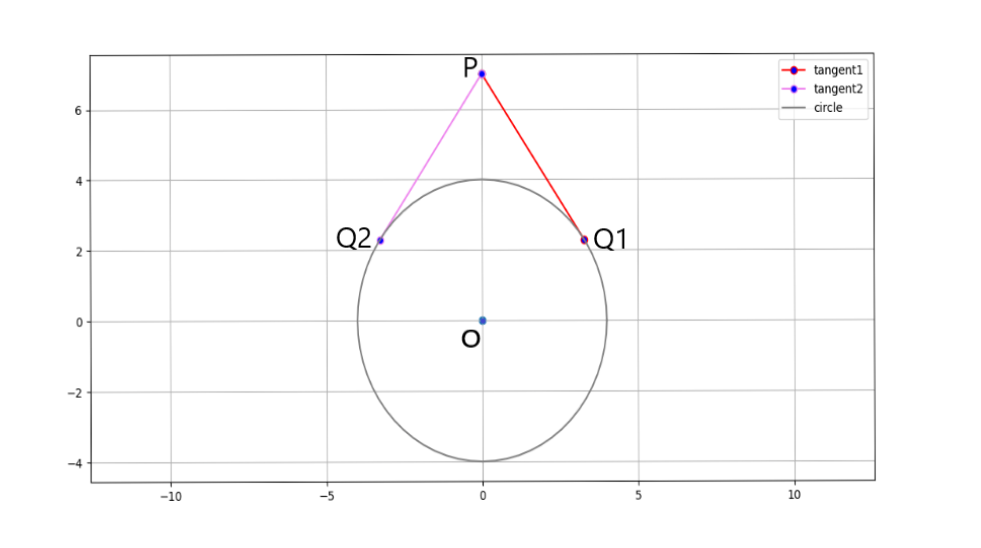
\includegraphics[width=\columnwidth]{imagePython}
	  \caption{}
	  \end{figure}
	  	  	  
\begin{itemize}

\item Calculating the length of tangent $PQ2$, which is the third side of the triangle OQ2P, right-angled at Q2 using the Pythogorean theorem using C. \\

\end{itemize} 
 
 \begin{figure}[h!]
	  \centering 
	  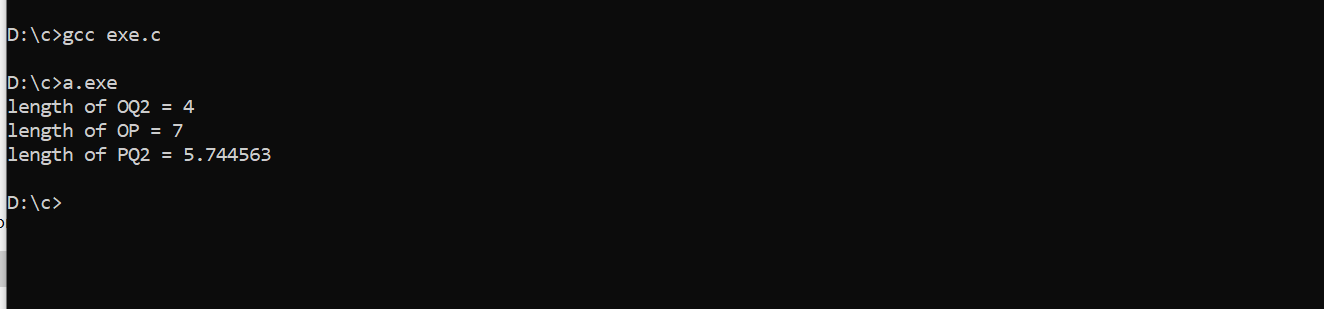
\includegraphics[width=\columnwidth]{imageC}
	  \caption{}
	  \end{figure}


\end{document}



